\documentclass[12pt,oneside,openright]{report}

\usepackage[utf8]{inputenc}
\usepackage[scaled]{helvet}
\usepackage{subcaption} % Add the subcaption package for subfigures
\usepackage{dirtytalk} %quoting package
\renewcommand\familydefault{\sfdefault} 
\usepackage[T1]{fontenc}
\usepackage{fancyhdr,xcolor}

\usepackage{graphicx} % Add the graphicx package for including images
\usepackage{geometry}
\usepackage{amsmath} % Add this line to your LaTeX preamble to use \text

\usepackage{pdfpages}
\usepackage{afterpage}
\usepackage{caption}
\usepackage{float}
\usepackage{xcolor}
\usepackage[style=authoryear,backend=biber]{biblatex}
\addbibresource{bibliog.bib}
\usepackage[colorlinks=true,linkcolor=black,anchorcolor=black,citecolor=black,filecolor=black,menucolor=black,runcolor=black,urlcolor=black]{hyperref}\usepackage{graphicx}
\geometry{
  a4paper,
  left=20mm,
  right=20mm,
  top=3cm,
  headheight=4cm,
  bottom=3.5cm,
  footskip=3cm
}

\renewcommand*{\bibfont}{\footnotesize}

\newcommand{\changefont}{
    \fontsize{18}{16}\selectfont
}
\definecolor{boxcl}{HTML}{1188BB}
\definecolor{tubred}{HTML}{1188BB}



\begin{document}

\begin{titlepage}
    \centering
    % Include the image with a width of one-third of the page
    
\includegraphics[width=0.5\textwidth]{Hu-logo.png}
    \vspace{2cm}
    
    {\huge \textbf{Multisensory Integration in Virtual Reality: Effects of Passive Haptic Stimulation}\par}
    \vspace{2cm}
    {\LARGE Master Thesis\par}
    \vspace{0.5cm}
    {\textbf{submitted in fulfillment of the requirements for the degree}\par}
    Master of Science (M.Sc.)\par
    {\textbf{in the master's program ``Mind and Brain''}\par}
    \vspace{1.5cm}
    {\textbf{Humboldt-Universität zu Berlin}\par}
    {\textbf{Berlin School of Mind and Brain}\par}
    \vfill
    \raggedright
    \begin{tabular}{ll}
        \textbf{Handed in by}: & Benjamin Dupré \\
        \textbf{Date of birth:} & 26.04.1986\\
       \textbf{ Address:} & Hoppestraße 16, 13409, Berlin \\
    \end{tabular}
    \vfill
    \begin{tabular}{ll}
        \textbf{1. Supervisor:}& Dr. Michael Gaebler \\
        \textbf{2. Supervisor:}& Professor Dr. Arno Villringer  \\
    \end{tabular}
    \vfill
    {Berlin, \today \par}
\end{titlepage}

\section*{1. Introduction}
%\subsection*{1.1 Problem \& Significance}

We have all heard at some point that our body behaves like an orchestra, with the brain as the conductor. Within this orchestra, multiple specialized musicians are organized together creating a melody grander than any individual musician could aspire to achieve alone. However, it's plausible that there is more than one orchestra coordinator, but rather a team of orchestra coordinators \parencite{Morten2021}. Recent findings suggest an unseen conductor outside the brain, providing subtle cues that dictate whether the symphony focuses on its harmonies or the audience's mood. This concealed orchestra director serves as an analogy for the role the heart cycle\footnote{Refers to the sequence of events that occur during each heart beat. Involving the contraction (systole) and relaxation (diastole) of the heart chambers} plays in signal perception and multisensory integration\footnote{Multisensory integration refers to the ability to synthesize information arriving from cross-modal stimuli}.

The heart cycle has become central to ongoing research in interoception\footnote{Interoception refers to the process by which the nervous system senses, interprets, and integrates signals originating from within the body, providing a moment-by-moment mapping of the body's internal landscape across conscious and unconscious levels.\parencite{Khalsa2017InteroceptionAM}}. The electrical discharge generated by the heart every pulsation, is transmited to the brian \footnote{The baroreceptor-mediated signals are transmitted through the glosso-pharyngeal and vagus nerves to the brainstem nuclei, reaching the nucleus tractus solitarii (NTS) and the parabrachial nucleus (PBN), where they are involved in the homeostatic control of blood pressure and heart rate.\parencite{SALTAFOSSI2023108642}} and there plays a significant role on how we process external stimuli (e.g. touch) \parencite{esra_p}. This influence is extensively observed in both psychophysics\footnote{The study of the relationship between the physical world and its sensory representations. Perceptual experiments often recruit only a few subjects; these subjects are highly trained, and each contribute a large number of observations. \parencite{KINGDOM2012234,WASKOM2019100}} and cognitive experimental setups\footnote{Cognitive experiments typically recruit larger samples, train for task comprehension rather than for expertise, and focus analyses on population-level parameters \parencite{WASKOM2019100}}. These findings constitute our initial set of facts, now we need an understanding of the operations performed by these findings \parencite{Barlow2012PossiblePU}. 

In this thesis, I propose a virtual reality (VR) experimental setup as a mechanism to generate this understanding. However, what are these findings preceisly? In the following section, I will mention some of these findings categorized into two groups: the psychophysical effects and the cognitive effects of the cardiac cycle. On a third section of the introduction, we look into the imporance of linking these findings in a ecological valid way \footnote{To sample stimuli or conditions in a way that respects the distribution and covariance of ecological variables if we hope to achieve generalizability beyond the boundaries of the experimental manipulation.\parencite{NASTASE2020117254}} and incorporating psychophysical findings and technics.

\subsubsection*{Psychophysical Heart Cycle Effects}

Psychophysical research looks into the relationship between physical phenomena and the perceptual effects they generate. These experiments are usually carried out with a single perceptual modality and high precision measurements. In heart cycle literature, stimuli is presented in sync with a specific cardiac phase (phase-lock). Findings show that the heart cycle plays a crucial role in diminishing or increasing our perception of external signals in touch, vision, and auditory cues \parencite{SALTAFOSSI2023108642}. In the somatosensory realm, the accuracy of detecting near-threshold stimuli showed a higher level during the diastolic phase of the cardiac cycle in contrast to systole \parencite{esra_p, AL2021118247, Grund643, motyka}. For vision and auditory stimuli, diastole improves accuracy and reaction time compared to systole \parencite{SALTAFOSSI2023108642}. However, real-life stimuli are rarely presented in a single modality. How does the heart cycle behave in multisensory situations?

Answering this, a recent study investigates multiple simultaneous sensorial modalities \parencite{SALTAFOSSI2023108642}. Explored the modulation of multisensory integration by the cardiac phase. Forty participants in good health performed a Simple Detection Task involving unimodal (Auditory, Visual, Tactile) and bimodal (Audio-Tactile, Audio-Visual, Visuo-Tactile) stimuli. These stimuli were presented either 250 ms after the R-peak of the electrocardiogram (systole) or 500 ms after (diastole). The study found a generalized impact of cardiac cycle phases on detecting both single and combined stimuli. Reaction times prove speedier for stimuli presented during diastole when contrasted with those in systole.

Additionally, this study utilizes the well-known Race Model Inequality (RMI) and response times (RT) to measure multisensory integration. In sensory modality testing, redundant signal effects refers to how individuals respond faster to redundant sensory signals compared to unisensory signals. One proposed explanation to the RSE model is Race Model Inequality (RMI). This model suggests that evidence for each signal is accumulated separately by parallel decision units (e.g. one for audition and one for vision) and that the first unit to reach its threshold triggers a response. 

Once again, the diastolic cardiac phase enhances the response to the sensory signal. The integration of Audio-Tactile and Visuo-Tactile stimuli showed higher integration when presented during diastole as opposed to systole, unlike Audio-Visual stimuli. This observation suggests a potential specificity in the influence of the cardiac phase on multisensory integration, particularly in stimuli involving somatosensory (e.g. tactile) inputs.

So far, all studies involve the passive presentation of stimuli and phase-locked conditions. It would seem that the role of the heart cycle as an orchestrator works under very specific circumstances, limited to the passive presentation of stimuli and locked to a particula heart cycle. In our day-to-day lives, stimuli comes to us in a constant stream, through multiple modalities; as well as, we actively seek specific stimuli. Would a more naturalistic stimuli interaction still show this cardiac phase influence?

\subsubsection*{Cognitive Heart Cycle Effects}

The second group of studies delves into higher cognitive functions. For instance, an illustrative study aims to measure if there's a difference in how we memorize a word presented during a specific cardiac phase. Words were shown within a limited attentional timeframe, synchronized with various cardiac cycle phases. This sought to investigate whether natural baroreceptor stimulation affects word detection and subsequent memory. The study reveals that recalling words presented during systole is lower compared to those presented at diastole. This memory decrease during systole is more pronounced for words identified with low confidence and heightened among individuals with lower interoceptive sensitivity, measured through a heartbeat counting task \parencite{Garfinkel2013-cy}.

Another two studies look to understadn if the way in which we actively sample the world is similarly modulated by the phase of the cardiac cycle. The first study focus lies on exploring the role of the heartbeat in active information sampling, investigating whether humans unconsciously arrange their environment to encounter pertinent signals during preferred cardiac phases. In the visual memory experiment's encoding phase, participants navigated through a series of emotional pictures, aiming to memorize them for a subsequent recognition test. Through self-paced key presses, they initiated the display of brief (100 ms) images. The study's findings unveil fluctuations in self-triggered picture onsets throughout the cardiac cycle, notably heightened during cardiac systole, yet without impacting memory performance. This leads the study to conclude that active information gathering incorporates signals related to the heartbeat.\parencite{Kunzendorf2019-vz}. A similar study confirm these findings. It was achieved by presenting participants with arrays to compare in size. They measured participants' eye movements, heart rate, and response times. The authors similarly found a significant coupling of saccades, subsequent fixations, and blinks with the cardiac cycle. They observed that more eye movement occurs during systolic phases while more fixation happens during diastolic phases, thus demonstrating an active perceptual role.\parencite{GalvezPol2018ActiveSI}.

So far, we've observed the influence of the heart cycle on perception, recognition, and active sampling. How do these pieces of information connect to the heart cycle's overarching function? Do they suggest an organizing role for the heart cycle? To draw an analogy, is the heart cycle akin to being part of the brain's team of orchestra conductors? If it is, what mechanism enables it to simultaneously influence such a wide array of functions?

\subsubsection*{Linking facts together}

As our understanding of the role of the cardiac cycle grows, the gaps between perception of external stimuli and cognitive functions widens. How does the heart cycle manage to influence diverse cognitive functions, such as word recognition and stimuli perception?

Several of the previously mentioned papers offer some explanation. Most point towards an interoceptive predictive framework . This framework posits that repetitive bodily signals, like the heartbeat cycle, can be predicted and suppressed to prevent entry into conscious perception, inadvertently leading to the suppression of external stimuli\parencite{AL2021118247, SALTAFOSSI2023108642,Allen2022}. 

Another paper formulates a complete computational interoceptive predictive framework \parencite{Allen2022}. This paper goes beyond by utilizing Markov Desicion Process. The Agents infer which policy they are persuing (relax or aroused) to produce the best mapping possible. The policies are defined operationally in terms of transitioning beween interoceptive states. For example, in relaxed state the shifts in probability among cardiac states result in two phases of diastole and one of systole. In contrast, arousal prompts an immediate transition from the initial diastolic state to systole. Essentially, arousal triggers cardiac acceleration and extends the average duration spent in systole. Its premise assumes that precise visual information is available only during specific phases of the cardiac cycle, contingent upon one's state of arousal. Among its findings, the paper demonstrates the model's ability to replicate various psychological and physiological phenomena found in the interoceptive inference literature. It provides a means to test such a model.

The models porvided so far are used to explain for stimuli presented during a specific heart cycle, in which we are influeced by our proprioceptive state. Although they would only account for exteroceptive suppression and offer no explanation as to how they link with behavioral or cognitive outcomes. At the moment this theories are in need of behavioral work since this provides understanding, whereas physiological interventions test causality\parencite{KRAKAUER2017480}.

To accomplish this, a more comprehensive experimental framework should encompass not just psychophysical stimuli but also broader cognitive functions extending beyond mere perception. Such tasks can help refine and assess an individual's strategies and level of involvement, minimizing the influence of uncontrolled higher-order processes \parencite{WASKOM2019100}. The initial phase of this approach involves replicating previous studies and aligning the experimental conditions more closely with real-world situations. This enhances the ecological validity and furthers our comprehension of how body-brain interactions manifest in human psychology \parencite{schmuckler2001ecological}. This process involves building on previous findings while integrating new experimental setups.

\subsubsection*{The Thesis}

We are proposing new experimental setup using Immersive Virtual Reality (IVR). IVR, known for its effectiveness in studying cognitive processes within controlled yet complex scenarios, traditionally relies on visual displays and head-hand movement tracking. We propose a setup using VR head-mounted displays with Electrocardiogram (ECG) and haptic devices. However, the integration of these devices presents new challenges, both practical and technical, as well as in terms of alignment with existing literature \parencite{Klotzsche2023}.

Particularly in the realm of psychophysical experimental setups, notable distinctions emerge. For instance, most studies in existing literature involve very brief periods of Reaction Time (RT). Due to the nature of IVR, RT tends to be considerably longer. Furthermore, IVR inherently involves multiple senses,  often involving visual, tactile, and proprioceptive senses and making all studies inherently multisensory. In contrast with most psychophysical studies that are multisensory. 

Therefore, the primary objective of this thesis is to validate the manipulation in the context of a multisensory heart cycle study. This is why the chosen study to mimic results is \textcite{SALTAFOSSI2023108642}, which is to my knowledge the only study looking into heart cycle and multisensory integration. Specifically to test the feasibility of manipulating touch within a heart cycle-IVR setups. To achieve this, one outcome is to assess the impact of passive haptic stimuli on reported immersion. Here the participats reported that the gloves increased the sense of inmertion, altough as not to have a relevant effect in the performance of the task. Additionally, the respone times (RT) showed a significant overall difference for the touch condition, thus validating the set up.

A secondary objective of this study is to to mimic the findings from \textcite{SALTAFOSSI2023108642}. Relevant for this study is the redundancy signal effect (RSE) and race model inequality (RMI). We observed that the overall performance partially adhered to the RSE, notably showing the congruent bimodal condition (V = T) significantly faster than the uni-modal condition (V). No significant differences were found between incongruent bimodal condition ($V \neq T$) and the single condition (V). Additinoally, when looking into the cumulative distibution functions (CDF) for different RT, we replicated the findings showing again faster bimodal conditions than unimodal conditions. Nonetheless, with potential violations specifically for the first 200ms

Considerable distinctions exist between the stimuli employed in this study and the referenced one. In this investigation, sole reliance resides upon vision as single modality, whereas the reference study has measurments for single modalities vision, touch and audio. Tactile in the reference study is determined for each participant with the method of the limits. In our study is simulated by a vibrotactile glove. Furthermore, this inquiry revolves around conditions primarily focused on the tactile sense\footnote{Touch, within this thesis, adopts an encompassing classification of tactile sensation, encapsulating five distinct modes predicated upon the presence or absence of voluntary movement: (1) tactile (cutaneous) perception, (2) passive kinesthetic perception, (3) passive haptic perception, (4) active kinesthetic perception, and (5) active haptic perception \parencite{Healy2003HandbookOP}}. For the scope of this thesis, touch specifically denotes passive haptic perception generated through a vibrational Data-Glove, compare to the reference study were is applied through a electrical current. Vibro-tactile stimu.lation significantly affected RT in participants and shows promising results for future heart-cycle analysis.

By probing the influence of passive haptic stimuli on response time within a motor-memory task, this study replicates the principal observations delineated in heart cycle multisensory integration literature \parencite{SALTAFOSSI2023108642}, thereby confirming in IVR as means of developing pschophysical investigation of cognition.

%I am Here at this point % I should jump to results and Discussion Section.

\section*{2. Methods}
\subsection*{Participants}
The call for participants targeted healthy, non-smoking German-speaking individuals between 18 and 30 years old. Initially, 23 individuals participated in the study, but ultimately, only 20 participants were included in the final sample. Among the three excluded individuals, two failed to complete all necessary questionnaires, while the third exceeded the age limit. Notably, a greater number of women (15) responded to the call compared to men (5). The average age across the sample hovered around 25 years, with a slight deviation observed in one participant ($\mu=25.1, \sigma=6.3$).

\begin{figure}[h]
    \centering
    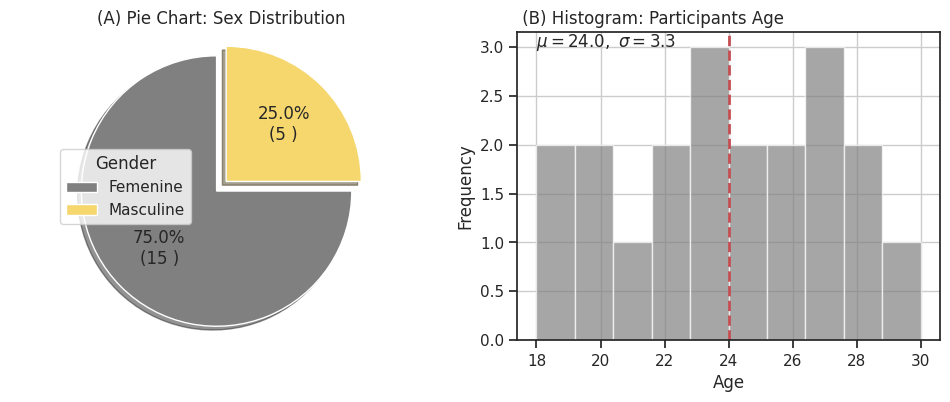
\includegraphics[width=12cm]{/home/perdices/Dokumente/Github/m-b_thesis/Analysis/figures/participants.png}
    \captionsetup{justification=justified, margin={2cm,2cm}, font={small}}
    \caption{Participants Composition}
    \label{fig:mesh1}
\end{figure}

    
\subsection*{Materials}
\subsubsection*{Electrocardiogram (ECG):}
Heart rate data was collected using an Arduino Uno and a SparkFun Single Lead Heart Rate Monitor - AD8232. The collected data is transferred through a USB 2.0 connection and integrated into the Unity log file at a frequency of 133 Hz. Compared to a clinical ECG, this device entails a serial interface that can send triggers via USB directly to a computer and software (e.g. Unity, Matlab) with minimal delay due to its architecture. Its software and hardware is open-source and publicly available \parencite{TimsECG}.

\subsubsection*{Head Mounted Display \& Lighthouses:}
The VR setup includes a HTC Vive head-mounted display (HMD) with two lighthouses. The headset specifications include a Dual AMOLED 3.6" diagonal display, with 1080 x 1200 pixels per eye (2160 x 1200 pixels combined), a 90 Hz refresh rate, and a 110-degree field of view. The lighthouses are equipped with SteamVR Tracking, G-sensors, gyroscopes, and proximity sensors. Both the HMD and lighthouses are connected using USB 2.0. For this study, the VR controllers were not used, and instead, hand tracking was performed using the Leap Motion sensor.

\subsubsection*{Leap Motion Controller:}
The Leap Motion Controller has a field of view of 150x120 degrees, with a variable range of roughly 80 cm (arm's length). It weighs 32 grams and is mounted on the HMD. The device features two 640x240 infrared cameras with a frame rate of 120 fps.

\subsubsection*{Data Gloves:}
The data gloves used in the study are equipped with magnetic sensors and connected to Unity using a microUSB connection. These gloves provide haptic feedback through 10 vibrotactile actuators, offering a wide range of tactile sensations with 1,024 levels of intensity. The gloves also incorporate complete finger tracking using six 9-axis Inertial Measurement Units (IMUs). These IMUs enable precise tracking of finger movements, allowing for accurate gesture recognition and enhanced interaction in virtual environments.


\subsection*{Task}

Participants after being debiref with Covid-Specific rules, information privacy and ethical norms recieved information about the experiment. Here they cosent and proceed to do all following tasks. It is important to mention that I did not made use of tasks\footnote{Original study VR/ECG-study Akbal/Villinger} since I have modified the original hypothesis the primary study set out to answer. Nontheless, since all participants included answered all questionaires and performed all tasks I report all of them. Not only the ones use in the analysis section 


\textbf{Questionnaires:} Before the IVR experience, participants completed the Edinburgh Handedness Questionnaire and the PRE-Cybersickness Questionnaire. Following the IVR experience, participants filled out the Virtual Reality Subjective Evaluation Questionnaire and POST-Cybersickness Questionnaire. Both Questionaires are included in the Appendix section.

\textbf{Heartbeat Count Task (HCT):} Participants performed a one-minute heartbeat count task before and after the IVR task. Note that this task is not considered within this thesis because of being out of the scope of this secondary study.

Following the completion of the initial questionnaires and HCT, participants moved to another room where the IVR  equipment was set up. This included a head-mounted display, data gloves, and an ECG device. Participants received a brief training session before proceeding with the heartbeat count task and the IVR memory-motor task.

\textbf{IVR Memory-Motor Task:} In Figure \ref{fig:looks}, two panels are depicted. On the left side of the figure Panel I, we observe the external view of a participant wearing the OVR, ready to commence the IVR Memory-Motor Task. Panel II on the right side of the figure showcases four out of the five steps participants undergo when initiating a trial set. These steps are outlined below:

\begin{enumerate}
    \item[\textbf{a.}] Participants stand in front of a virtual table, allowing ample time to acclimate to the virtual environment, as depicted in Figure \ref{fig:looks}. When they feel prepared, the session commences as they calibrate by placing their hands on the virtual table.
    \item[\textbf{b.}] Prior to each trial within every set, a new calibration process begins. Participants place their palms facing up within the shadowed hands, ensuring standardized positioning. Refer to Figure \ref{fig:looks} (b) for the calibration setup.
    \item[\textbf{c.}] Once the calibration is complete, a two-dimensional sketch appears in front of them (Figure \ref{fig:looks} (c)), prompting them to memorize the red ball's position. Participants then observe a template on the table, resembling the initial sketch they memorized. Their task is to place the ball swiftly and accurately in the correct location on the template. In the memory-sketch, the relevant position of the ball is denoted by the red circle. During this phase, participants keep their virtual hands open with palms facing up.
    \item[\textbf{d.}] As soon as the memory-sketch disappears, a red ball appears in either the left or right hand of the participants. Simultaneously, a vibration could start in the glove. The vibration may or may not match the visual location of the red ball. If the vibrating hand matches the visual location of the ball, the condition is congruent ($V=T$). If the vibrating hand does not match the visual location of the ball, then the trial is incongruent ($V \neq T$). If there is no vibration at all, the condition is purely visual ($V$).
    \item[\textbf{e.}] After placing the ball on the template, the ball and template disappear. 
\end{enumerate}

\begin{figure}[!ht]
    \centering
    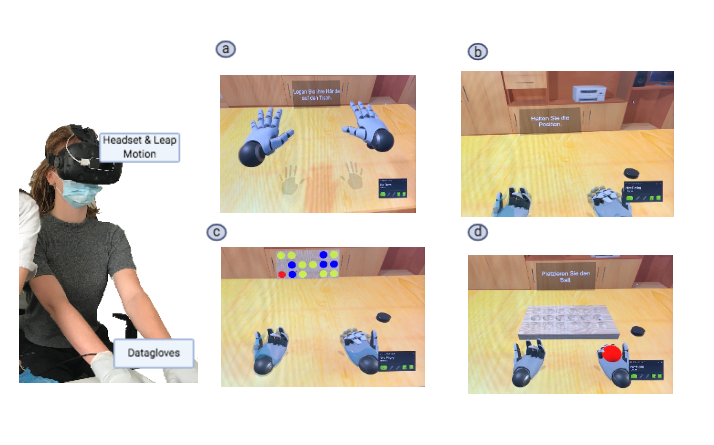
\includegraphics[width=15cm]{/home/perdices/Dokumente/Github/m-b_thesis/Analysis/figures/design_ilustration.png}
    \put(-420,240){\textbf{I}} % Adjust (-20,340) to position "I" label as desired
    \put(-320,240){\textbf{II}} % Adjust (360,340) to position "II" label as desired
    \captionsetup{justification=justified, margin={2cm,2cm}, font={small}}
    \caption{Illustration of the IVR Memory-Motor Task: Panel I show a participant wearing equipment. Panel II shows step (a) represents the acclimation period during initial setup and first step calibration; (b) showcases the first-person perspective of the second calibration phase; (c) displays the 2D sketch for memorizing ball position; (d) presents the appearance of the ball and the 3D template for ball placement, marking the beginning of each trial.}
    \label{fig:looks}
\end{figure}
 
In a sequence of 108 trials, three conditions—congruent ($V=T$), incongruent ($V \neq T$), and visual-only ($V$)—were presented randomly and rapidly, each occurring 36 times. Each trial commenced upon positioning the ball in a hand, concluding only upon its precise placement on the designated template (refer to Figure \ref{fig:looks}). 

Given that an IVR task inherently involves proprioceptive signals\footnote{Proprioceptive signals arise from our own actions, encompassing signals related to limb and trunk position and movement, sensations of effort, force, and heaviness. Proprioceptive receptors are situated in the skin, muscles, and joints. Information regarding limb position and movement doesn't stem from individual receptors but from clusters of afferents\parencite{Proske2012ThePS}.}, all conditions in the experiment integrate these signals and are thus multimodal. Consequently, the 'visual only' condition doesn't align with the unimodal classification commonly used in psychophysics literature. Nonetheless, for the sake of easier comparison to this literature in this thesis, I will refer to it as unimodal, and the congruent and incongruent conditions as bimodal.


\subsection*{Mesurements}
\subsubsection*{Immersive Virtual Reality (VR):}

 Movement data from the data gloves, Leap Motion device, and the HMD was collected. For movement analysis, only the wrist movements tracked by the Leap Motion device were considered, excluding the fingertips' magnetic tracking sensor data. All movements were recorded in a Euclidean coordinate system (X, Y, Z) with the original calibrating point set at (0, 0, 0). This provided a total of nine streaming sources of data (e.g., Headset X, Headset Y, Headset Z, and so on). Notably, rotational data was not included in the analysis.

Additionally, in the game output data, there are flags that signal if a button was pressed, if the ball is placed in the holder, and when the trial started.

\subsubsection*{Questionnaires:}
Both of the described questionnaires are included in the appendix of this thesis for further reference.

\begin{enumerate}
\item[(i)] \textbf{Virtual Reality Subjective Evaluation Questionnaire:} This self-designed questionnaire comprises 26 items aimed at assessing the sense of reality experienced during the VR session. It explores factors like engagement level, hand movement, task difficulty, and other controlling aspects. Participants responded using a Likert scale ranging from one to seven.

\item[(ii)] \textbf{PRE/POST-Cybersickness Questionnaire:} This study employs a shortened version of the simulator sickness questionnaire (SSQ) \parencite*{avpsy}. It utilizes a Likert scale ranging from one to four, featuring labels such as "not present," "somewhat," "clearly," and "very strongly." The questionnaire consists of 16 items, gauging symptoms like "fatigue" and "general discomfort," among others.
\end{enumerate}


\subsection*{Data Analysis}

\subsubsection*{Questionnaire}
The analysis of the questionnaire responses aimed to explore the impact of haptic gloves on reported immersion and related perceptions. Initially, the raw questionnaire data collected from 20 respondents, consisting of 27 questions rated on a scale from 1 to 7. Missing values were checked and handled appropriately, thus leaving us with 19. Statistical analysis included the calculation of descriptive statistics such as median ($\text{Mdn}$), mean ($\mu$), and standard deviation ($\sigma$) for each question. These statistics were instrumental in understanding the central tendencies and variability in respondents perceptions. A full view of all answers can be found in the Supplements section. 

\subsubsection*{Response Time}
All response times from the ball's entry into the scene until its disappearance were measured. Trials where the error button was pressed were excluded from the analysis. Prior to analysis, outliers were corrected by eliminating data points deviating more than 3 times the median absolute deviation (MAD), which is equivalent to 3 standard deviations assuming a normal distribution \parencite{Innes2019ACA}. Responses were not eliminated for being too fast; however, 13\% of trials were excluded due to excessive slowness. The final sample comprised 1826 response times (approximately 24 per condition per participant). Subsequent to the removal of outliers, the response times for each condition were transformed into rates (1/RT).

The transformation method entails the inversion of the RT and aligns with prior studies \parencite{Innes2019ACA}. However, this transformation method is not exempt from criticism \parencite{Lo2015-fv}. This study prioritizes normality in error distribution over other factors such as property scale or interacting effects. This prioritization allowed for the direct application of repeated measures ANOVA within subjects. Yet, when the ANOVA results were ambiguous, a General Linear Mixed-Effect Model (GLMM) was additionally applied, as recommended \parencite{Lo2015-fv}. Although this analysis is not present in the reference study, the utilization of GLMM aims to provide clarity regarding the significance of the conditions and the study's power.

To allow comparisons with Saltafossi's reference paper, the primary goal was to confirm the established redundant signal effect—indicating faster response times to bimodal stimulation compared to single stimulation—and partially construct the Race model Inequality to assess its applicability across all time periods $t$.

The experimental approach followed methodologies outlined in \cite{Ulrich2007,Innes2019ACA}. Operating with one individual and two bimodal stimuli mandated a simplified version without the "bounding sum." This omission precluded the creation and analysis of the violation frontier due to the absence of the Touch alone condition, reserved for inclusion in future experimental designs.

In consideration of this, the process involved generating empirical cumulative density functions (CDFs) for three conditions—Bimodal pairs ($F_{V=T}$, $F_{V \neq T}$), and Single Signal ($F_V$). Subsequent steps included percentile determination and aggregation across participants through paired t-tests at each scrutinized percentile. For a comprehensive breakdown and reference code, consult \cite{Ulrich2007}.

\section*{3. Results}
\subsection*{3.1 Assessing the Impact of the Haptic Glove on Reported Immersion}
    
Nineteen respondents answered 27 questions, rating them on a scale from 1 (Does Not Apply) to 7 (Totally Applies). The key findings from the questionnaire are as follows:
    
\begin{enumerate}
    \item In question number 24, the perceived increase in immersion due to the haptic gloves was high ($\text{Mdn} = 6$, $\mu = 6$, $\sigma = 0.76$). Furthermore, the task was considered enjoyable at least some of the time ($\text{Mdn} = 6$, $\mu = 5.4$, $\sigma = 1.04$).
        
    \item Question 26 revealed that haptic feedback was perceived as either not significantly improving performance or having a neutral effect ($\text{Mdn} = 3$, $\mu = 3.6$, $\sigma = 1.49$). Similarly, in question 12, the perception of haptic feedback improving response time was generally rated as neutral to not applicalbe ($\text{Mdn} = 3$, $\mu = 3.7$, $\sigma = 1.74$). In question 7, when asked about the impact on results, haptic feedback was perceived as not applicable ($\text{Mdn} = 6$, $\mu = 6$, $\sigma = 0.76$).
    
    \item Notably, the assertion that it was very challenging to remember the position of the red ball ($\text{Mdn} = 2$, $\mu = 2.9$, $\sigma = 1.45$) was generally disagreed upon. Conversely, in question 8, which asked the inverse question about the ease of remembering the location of the red ball ($\text{Mdn} = 5$, $\mu = 5.1$, $\sigma = 1.37$) allign with its counterfactual. 
    
    \item The highest variance was observed in question 13 ($\text{Mdn} = 5$, $\mu = 4.2$, $\sigma = 1.79$), indicating that haptic feedback made it easier to place the ball. Similarly, question 18, which inquired about the ease of counting heartbeats at the beginning of the experiment, also showed significant variance ($\text{Mdn} = 4$, $\mu = 4$, $\sigma = 1.79$). 
        
\end{enumerate}
    
Overall, participants reported increased immersion and enjoyment as a result of the added gloves. However, there was no perceived enhancement in response attributed to the presence of the gloves. The overall task was considered easy. Moreover, the notably high variance observed in the last two questions may suggest potential confusion among participants regarding these specific queries or significant individual differences in experiences. For a more detailed breakdown, please refer to the supplementary section.
    
\subsection*{3.2 Influence of Touch Stimuli on Response Time}
\subsubsection*{3.2.1 General Performance}

First, I examined the mistake rates in ball placement per condition to ensure they did not significantly affect the experiment. The mistake rates were as follows: visual-only condition ($V$) - $6.35\%$ ($\pm 0.99\%$, SEM); visual incongruent touch condition ($V \neq T$) - $5.79\%$ ($\pm 0.59\%$); visual congruent touch condition ($V=T$) - $6.91\%$ ($\pm 1.93\%$). However, a one-way ANOVA (feedback type) showed no significant effects ($ F \leq 0.08$, $p \geq 0.91$). Despite the task's complexity beyond mere stimulus recognition, these mistake rates remained notably low and were not further analyzed.

To investigate whether the experimental manipulations mirrored the well stablished result of Redundancy Signal Effect (RSE) studies, I conducted a one-way repeated-measures ANOVA. The test revealed a significant main effect for the stimulus ($F(2,38) = 3.4$, $p \leq 0.043$, $\eta p^2 = 0.15$). The median response time for the 'Congruent' condition ($V=T$) was the fastest ($3236$ ms $\pm 456$ ms), followed by the 'Incongruent' ($V \neq T$) condition ($3268$ ms $\pm 470$), while the slowest was observed in the absence of haptic stimuli 'None' ($V$) ($3284$ ms $\pm 463$). Thus, the experimental conditions significantly influenced response times, as illustrated in Figure \ref{fig:error}.

\begin{figure}[!ht]
    \centering
    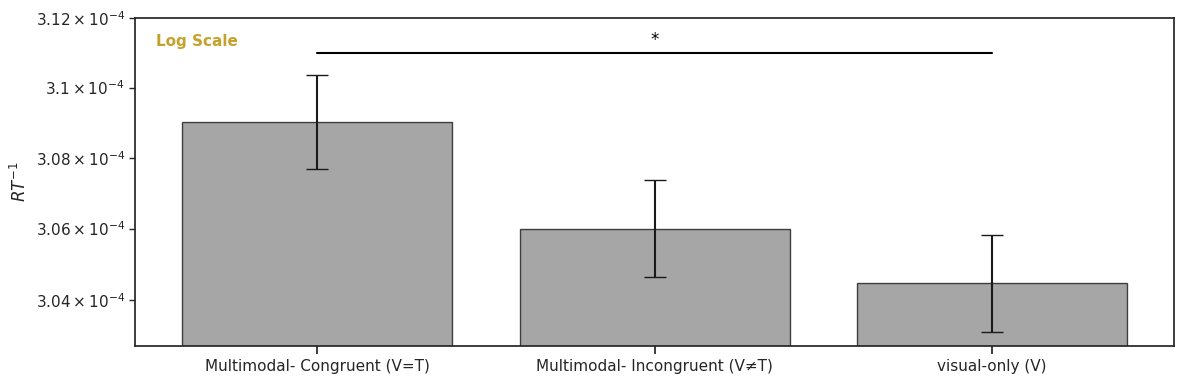
\includegraphics[width=12cm]{/home/perdices/Dokumente/Github/m-b_thesis/Analysis/figures/bar_erros_bars_stimulus_constructions.png}
    \captionsetup{justification=justified, margin={2cm,2cm}, font={small}}
    \caption{One-way repeated-measures ANOVA using $RT^{-1}$. The test revealed a significant main effect for the conditions ($F(2,38) = 3.4$, $p \leq 0.043$, $\eta p^2 = 0.15$)}
    \label{fig:error}
\end{figure}


However, post hoc Tukey HSD tests did not reveal any specific pairwise differences. While an overall difference among conditions was observed, specific pairwise differences were not identified.

Given the absence of identified specific pairwise differences in the post hoc analysis, I conducted a more comprehensive investigation using a Generalized Linear Mixed Model (GLMM). While not employed in the referenced paper, this method offers numerous advantages in multilevel research designs. It addresses the following issue stated by \textcite{Lo2015-fv}: 

"A linear relationship between the standard deviation of RTs and mean RT demonstrated in many previous studies of RT in binary choice tasks. This linear relationship is also evident in plots of the residuals, indicating heteroscedasticity in LMM analyses, characterized by an increasing spread in residuals for longer predicted RT."

As I will delve into further in the Discussion section, this issue suggests that the statistical power required for tasks involving longer Immersive Virtual Reality (IVR) times needs to be significantly higher compared to psychophysical experimental setups. An alternative approach, as mentioned by the author, is to utilize GLMM.

By using GLMM, instead of imposing normality and eliminating error deviation, we allow the use of distributions that match the properties of the measured RT \parencite{Lo2015-fv}. I utilized the \textit{statsmodels} statistical package in Python, specifically the \textit{mixedlm} function, similar to other studies \parencite{RSE_FBI}.

The mixed linear model analysis aimed to assess the impact of feedback types (($V=T$), ($V \neq T$), ($V$)) on response times. The model included feedback type as a fixed effect and participant as a random effect, with the 'Congruent' feedback type serving as the reference category.

The model coefficient for the 'None' ($V$) feedback type ($\beta = 45.726, SE = 22.594, p = 0.043$) reached statistical significance at the conventional level ($\alpha =0.05 $) when compared to the 'Congruent' ($V=T$) feedback type. This suggests a significant difference in response times between the 'None' and 'Congruent' feedback types. The coefficient for the 'Incongruent' feedback type ($\beta = 32.975, SE = 22.686, p = 0.146$) did not reach conventional levels of significance.

Thus, the 'Congruent' condition demonstrated significantly faster performance compared to the visual-only condition. This outcome aligns with the expected results according to the RSE. However, the findings present a mixed perspective. Despite this significant contrast, the more stringent post hoc Tukey HSD tests revealed no notable differences between pairwise conditions. Additionally, the GLMM indicated significance solely between the 'Congruent' and visual-only ($V=T$ - $V$) conditions and not between the 'Congruent' and 'Incongruent' conditions ($V=T$ - $V \neq T$). To understand if this mixed results are due to the irrelevancy of the 'Incongruent' condition ($V \neq T$) or the result of changed behavior over time, we can investigate the looking at our CDF analysis.

\subsubsection*{3.2.2 Race Model Inequeality}

As already mentioned in the methods section, the experiment does not allow for a full test of the RMI, since originally the experiment did not consider tactile only condition. However, I will use the CDF from the model, assess the significance of their differences, and establish comparisons among the three experimental conditions. We observed that the overall performance partially adhered to the RSE, notably between the 'Congruent' and visual-only ($V=T$ ; $V$) conditions, but no significant differences emerged between the 'Congruent' and 'Incongruent' conditions ($V=T$ ; $V \neq T$). 

To mimic the results from \Cite{SALTAFOSSI2023108642}, I conducted a series of t-tests using individual participant data for the Gx, Gy, and Gz values at each percentile level. Rather than examining areas under the curve, I focused on the raw values of Gx, Gy, and Gz. Furthermore, instead of emphasizing time bins, I opted to discuss percentile levels, given the differing time ranges compared to traditional RMI literature. 

When comparing differences between Gx and Gy ($V$ ; $V \neq T$), no significant p-values were found for any percentile. The results between Gx and Gz ($V$; $V=T$) are presented in Table \ref{tab:response-time-range}. This table illustrates the results for all time frames and percentiles. Notably, significant differences emerged between Gx and Gy from percentile 16 onwards. Interestingly, for this percentile (as depicted in Figure \ref{fig:CDF}), the single modality visual ($V$) appears to be faster than the bimodal incongruent condition ($V \neq T$), suggesting a potential violation of the RSE. Conversely, subsequent results align with our expectations from the RSE. It's essential to note that when considering the distribution of all response times, the highest density is observed between 3100 and 3200 ms, encompassing over one-third of all answered trials.
 
\begin{table}[!ht]
    \centering
    \begin{tabular}{ccccc}
    \hline
    \textbf{Gx Time Range (ms)} & \textbf{Gx Min Max Diff (ms)} & \textbf{Percentile Estimation} & \textbf{T-value} & \textbf{p-value} \\ \hline
    (3070, 3621) & 551 & 10  & 1.19 & 0.12 \\
    (3078, 3626) & 548 & 13 & 1.31 & 0.1  \\
    (3084, 3648) & 564 & 16 & 1.88 & 0.04* \\
    (3086, 3687) & 600 & 19 & 2.04 & 0.03* \\
    (3087, 3708) & 621 & 20  & 2.01 & 0.03* \\
    (3092, 3748) & 656 & 23 & 1.97 & 0.03* \\
    (3094, 3760) & 665 & 26 & 2.06 & 0.03* \\
    (3098, 3766) & 668 & 29 & 2.03 & 0.03* \\
    (3099, 3768) & 668 & 30  & 2.02 & 0.03* \\
    (3104, 3814) & 709 & 33 & 2.11 & 0.02* \\
    (3106, 3838) & 732 & 36 & 2.08 & 0.03* \\
    (3111, 3846) & 735 & 39 & 1.83 & 0.04* \\
    (3114, 3848) & 734 & 40  & 1.79 & 0.04* \\
    (3119, 3861) & 741 & 43 & 1.74 & 0.05* \\
    (3121, 3907) & 786 & 46 & 1.55 & 0.07  \\
    (3123, 3969) & 846 & 49 & 1.36 & 0.09  \\
    (3124, 3978) & 855 & 50  & 1.33 & 0.1   \\
    (3130, 4171) & 1041 & 60  & 1.25 & 0.11  \\
    (3141, 4352) & 1211 & 70  & 1.21 & 0.12  \\
    (3153, 4645) & 1492 & 80  & 1.47 & 0.08  \\
    (3176, 4948) & 1772 & 90 & 0.53 & 0.3   \\ \hline
    \end{tabular}
    \captionsetup{justification=justified, margin={2cm,2cm}, font={small}}
    \caption{T-test results between Gx \& and Gz conditions. Response Time Range (ms), Difference RT (ms), Percentile Estimation, T-value, and p-value for each Percentile using the results of t-tests. * indicates significant p-values.}
    \label{tab:response-time-range}
\end{table}


\begin{figure}[!ht]
    \centering
    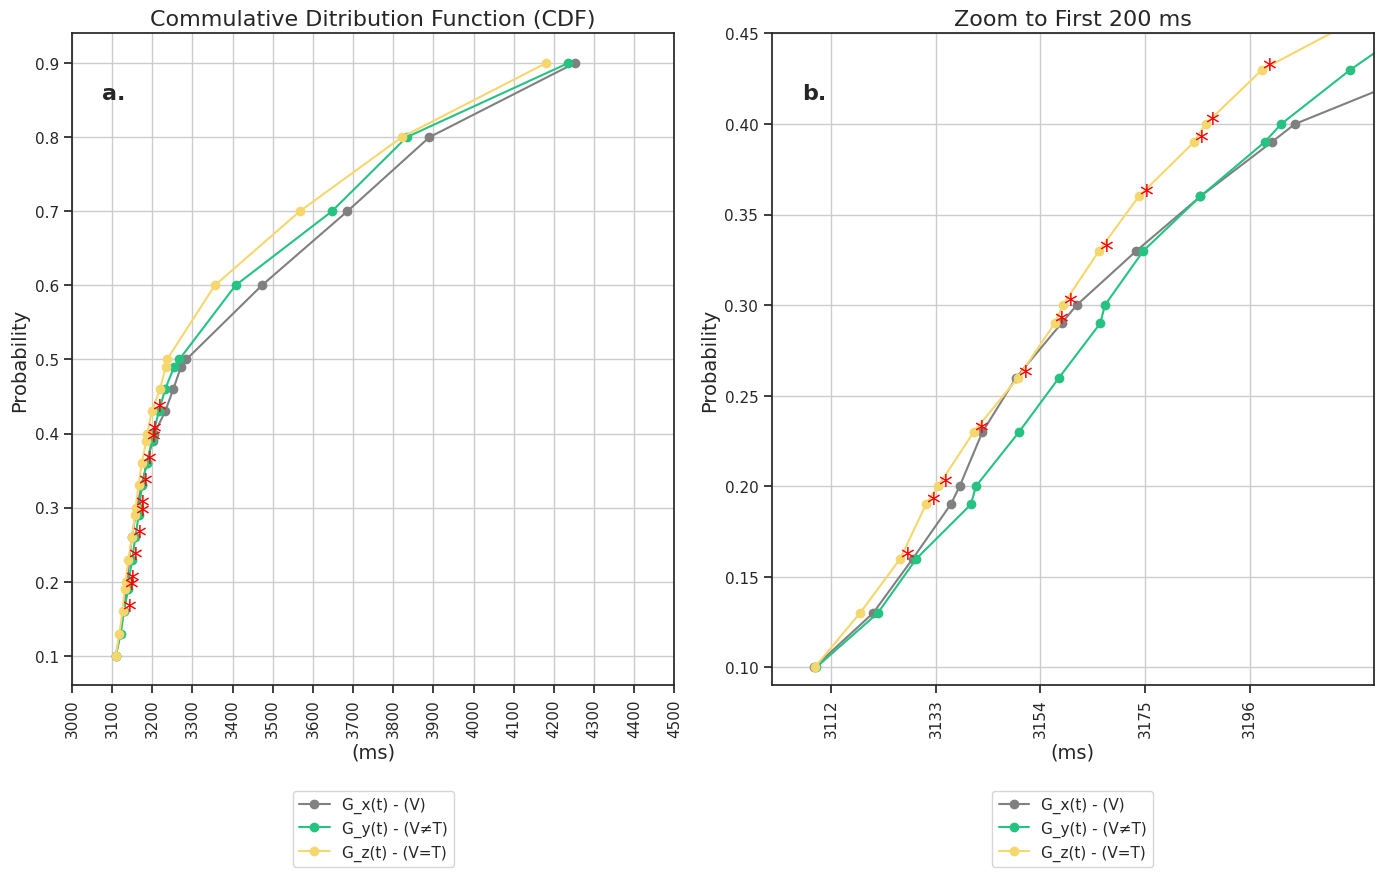
\includegraphics[width=15cm]{/home/perdices/Dokumente/Github/m-b_thesis/Analysis/figures/CDF.png}
    \captionsetup{justification=justified, margin={2cm,2cm}, font={small}}
    \caption{ (a.) Displays the 10 estimated percentile points for each of the three functions of interest: Gx, Gy, Gz, considering all participants. (b.) Is a zoom in the first 100 ms. Acording to the RSE, the visual $V$ type should be under Gy, Gz at all moments. Our data shows that is not the case for the RT in the first 200 ms.}
    \label{fig:CDF}
\end{figure}


\section*{4. Discussion}

This thesis aimed to test the feasibility of using IVR to study how the cardiac cycle modulates cognition and to bridge the gap between cognitive and psychophysical research. To achieve this goal, the thesis used an IVR memory task where participants had to remember a location and immediately place a red ball over this location in a 3D template. The condition was desgined so that  a passive vibro-tactile stimuli was activated along with the ball being presented into either matching the visual location of the ball or in the opposite hand. The study employed a within-subject experimental design with three categories: congruent visual-tactile stimuli, incongruent visual-tactile stimuli, and visual-only stimuli. The measured parameters were Reaction Time (RT) and Accuracy.

To establish a comparison, I followed the steps outlined in my reference study \parencite{Innes2019ACA, SALTAFOSSI2023108642, Ulrich2007}. It's important to note that there is only a single modality stimuli ($V$), limiting the possibilities of RMI comparisons.

The initial step involved testing the validity of stimulus construction by analyzing and modeling reaction times to uni-modal and bi-modal stimuli. Results were mixed. Overall, a significant difference between the conditions existed. While attempting to identify pairwise differences through a Tukey HSD test, no significant differences were found. However, a GLMM showed a significant difference between the visual-only ($V$) and visual-touch congruent ($V=T$) conditions. No significant differences were found between the incongruent ($V \neq T$) and the visual-only ($V$) conditions. These results confirmed the well-observed RSE in virtual reality during a ball positioning task and raised questions about the incongruent condition.

Analyzing the RMI reveals that the most frequently occurring RT falls between 3100 ms and 3200 ms, with over one-third of all trials within this 100 ms range. Additionally, when performing a t-test for all participants, the cumulative functions for each condition (Gx and Gz values) were significantly different only within this 100 ms period, not before or after. It's important to note that although the difference between Gx and Gy was not significant, for this 100 ms period, a potential violation of the RSE principle was observed, where a bimodal condition ($V \neq T$) was slower than a unimodal condition ($V$).

Descriptively, the same relationship between the visual-only ($V$) and the congruent condition ($V=T$) holds throughout the entire range of RT, in accordance with the RSE. However, this is not the case for RT between the incongruent condition and the visual-only condition, where the visual-only condition is faster than the incongruent condition ($V \neq T$) for the first 100 ms of the trial, violating the RSE. Later, the incongruent condition is faster than the unimodal visual-only condition, as expected with the RSE.

\Cite{RSE_FBI} proposes a plausible explanation for the absence of a difference in the RSE between congruent and incongruent conditions. It suggests that the mere simultaneous occurrence of visual and vibrotactile stimuli might suffice for multisensory integration, irrespective of whether these multisensory stimuli are functionally linked at a higher level or not (e.g., touch in the hand holding the ball).

An alternative explanation may relate to the context invariance assumption, which states that the processing of one signal is not affected by another.

The discrepancy observed in the incongruent case may be so marginal that the statistical power of the present study might not be sufficient to detect it significantly. Regarding the power of the study, one conclusion is that, due to considerations of ecological validity, each trial in our IVR study spans a longer time frame compared to traditional psychophysics experiments (with a mean duration of 3400 ms as opposed to the typical 200 ms). This extended duration contributes to increased variance and skewness in response times (RT). Moreover, according to the literature, the influence of the cardiac cycle on stimuli ranges from 10 to 40 ms, posing a challenge when investigating its effects in IVR environments. Consequently, the statistical power of future research needs to be increased threefold, considering, for instance, involving 60 participants, especially if an additional condition related to cardiac cycles is to be included in the analysis.



\newpage
\section*{Supplement}
    \begin{figure}[H]
        \centering
        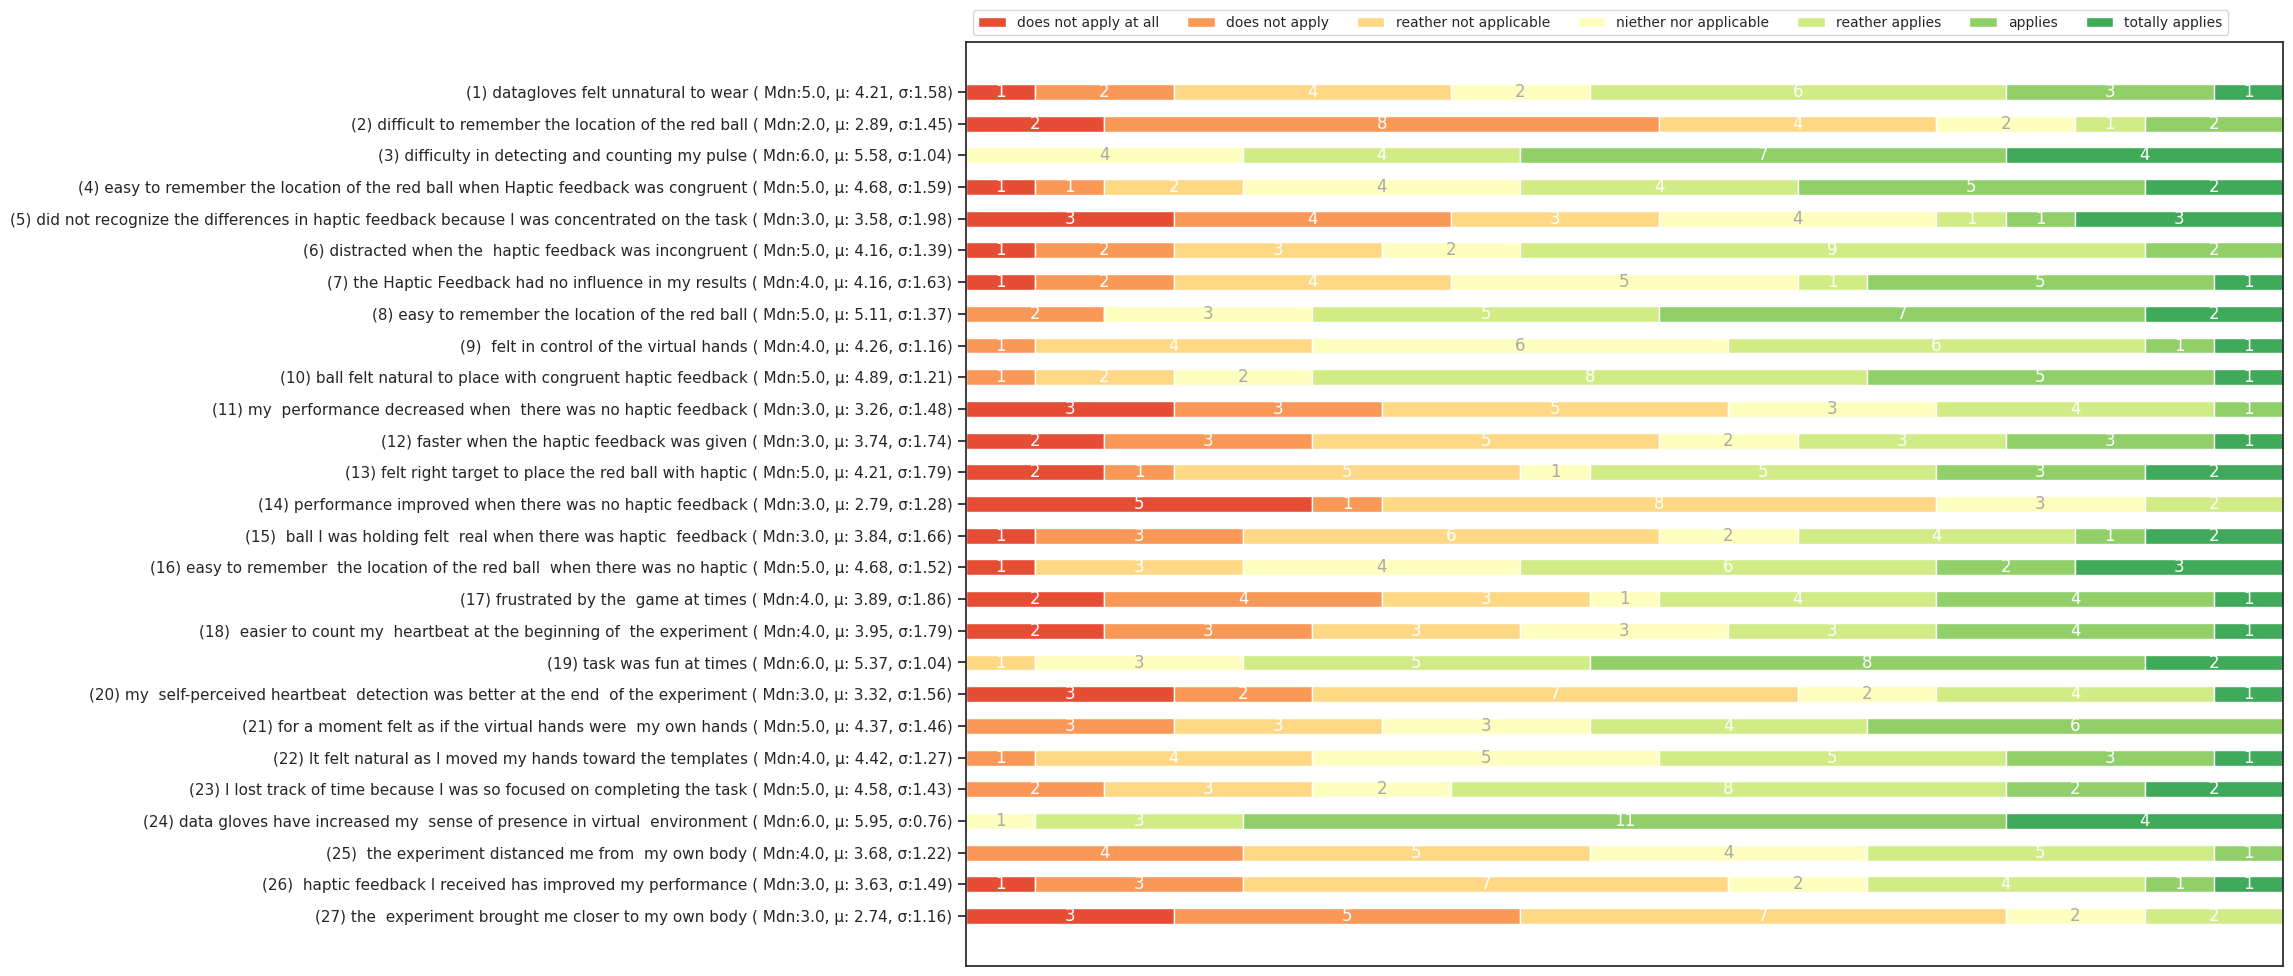
\includegraphics[angle=90, width=\textwidth, height=20cm, keepaspectratio]{/home/perdices/Dokumente/Github/m-b_thesis/Analysis/figures/questionaire_fig.png}
        \captionsetup{justification=justified, margin={2cm,2cm}, font={small}}
        \caption{Results: Virtual Reality Subjective Evaluation Questionnaire}
        \label{fig:quest}
    \end{figure}
\pagebreak


%-------- CREATING BIBLIOGRAPHY

\paragraph{\textbf{References}}
\printbibliography[heading=none]

%-------- CREATING Apendix

\pagebreak
\vspace*{\fill}
\section*{\centering Additional Material}
\vspace*{\fill}



\end{document}

